\subsection{Генерация отчетов}
Модуль генерации отчетов является одной из самых сложных частей системы, в связи с чем
он нуждался в особо тщательном проектировании, учитывающем все особенности поставленных задач
и возможность внесения изменений.

При разработке архитектуры модуля принято решение использовать наследование
для выделенения общих частей для отчетов по VOD и Live, так как большая часть
логики для них идентична, а различие состоит только в наборе показателей, а также
в наборе дополнительных параметров в форме отчета.

Таким образом контроллеры, классы форм отчета и построители образуют иерархии, в которых
определены базовые классы с общей логикой, а для каждого из типов отчетов (Live/VOD) реализованы
классы-наследники, специфицирующие части характерные для каждого из них.

\subsubsection{Формы отчетов}
Формы отчетов --- это классы, инкапсулирующие данные с параметрами отчета, 
в них реализованы методы для загрузки параметров из HTTP-запроса, а также для
сохранения значений в базу данных, для того, чтобы параметры отчета сохранялись
в рамках сессии конкретного пользователя.

\begin{figure}[!ht]
\begin{center}
\vspace{-0.4cm}
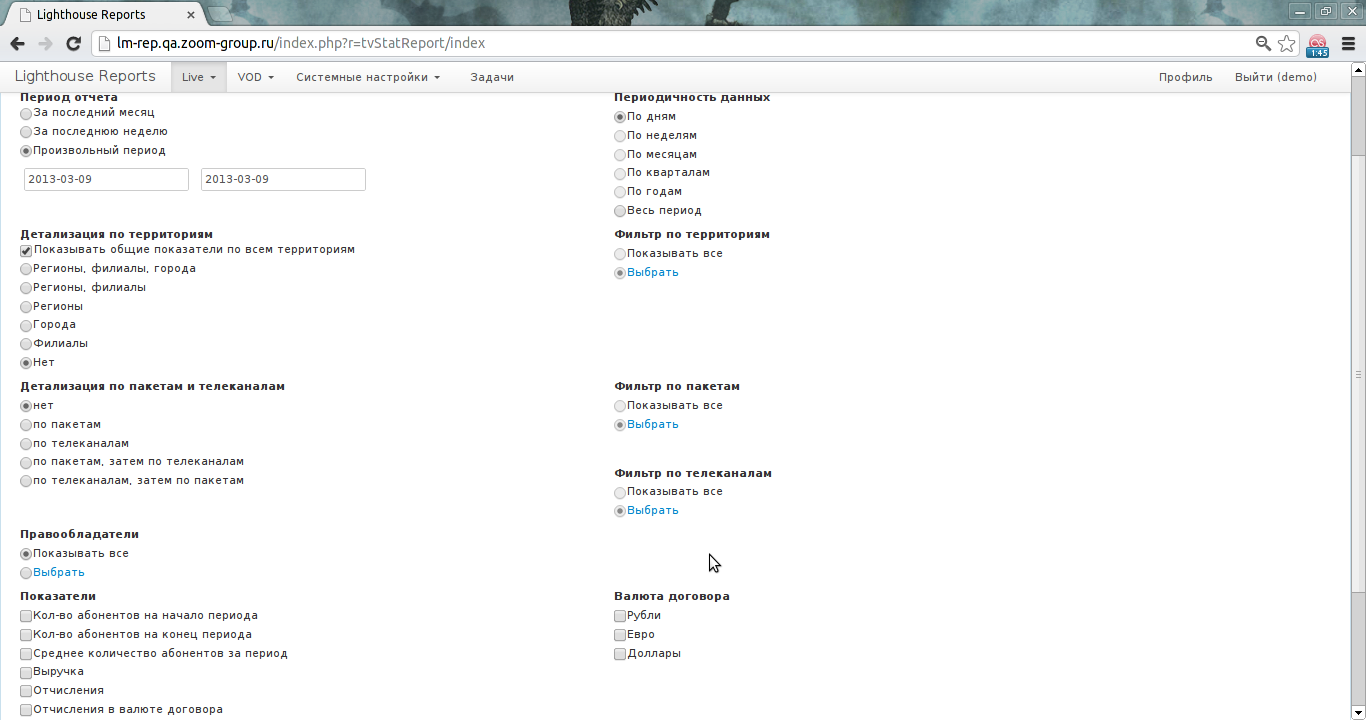
\includegraphics[scale=0.5, trim=00mm 00mm 200mm 00mm, clip]{../resources/lm_screen.png}
\caption{Форма параметров отчета}
\label{gr:report_form}
\end{center} 
\end{figure}

\subsubsection{Структура отчета}
\begin{figure}[!ht]
\begin{center}
\vspace{-0.4cm}
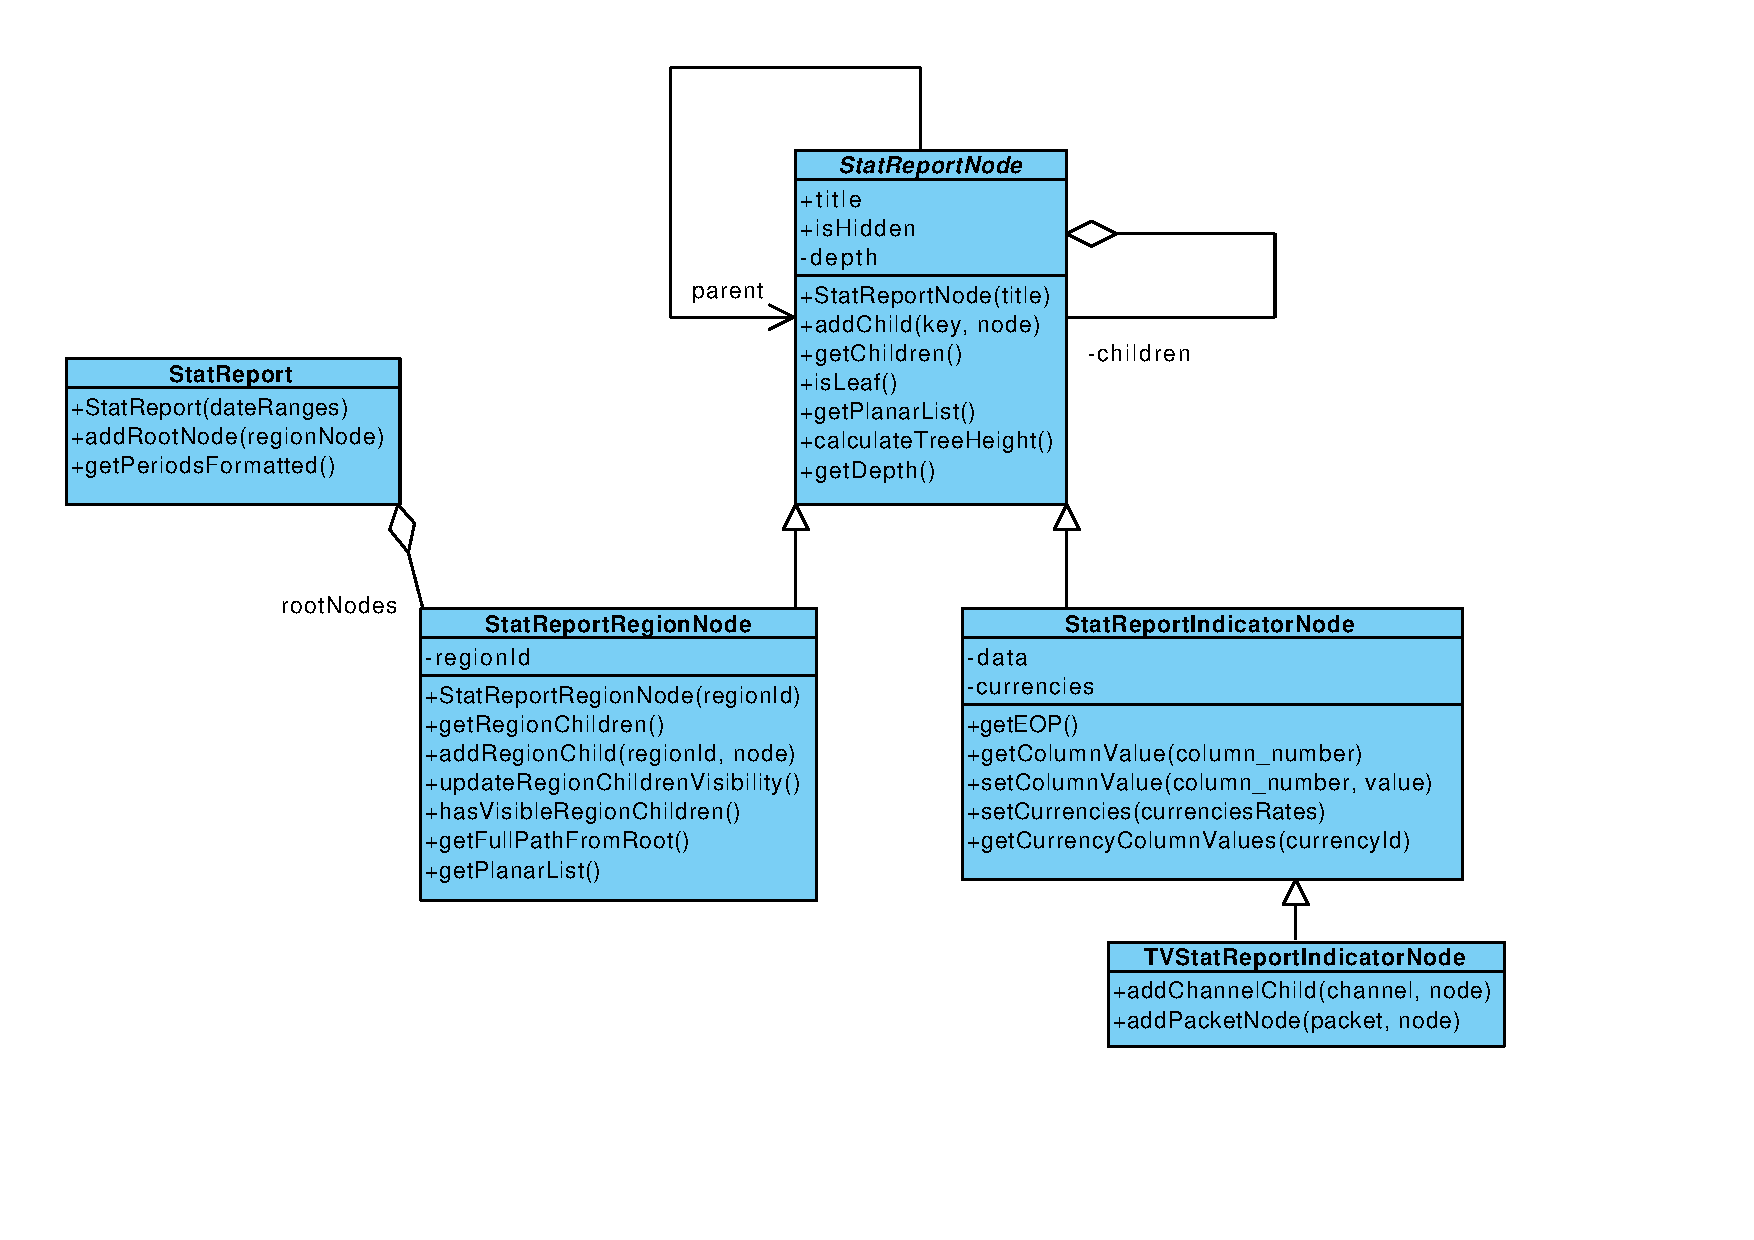
\includegraphics[scale=0.65, trim=00mm 25mm 00mm 10mm, clip]{../resources/uml/StatReport.pdf}
\caption{Диаграмма классов, составлящих структуру отчета}
\label{gr:report_structure}
\end{center} 
\end{figure}
На рис. \ref{gr:report_structure} изображена структура отчета в виде диаграммы классов его элементов.

Как описано в разделе \ref{section:stat_reports_task}, отчеты представляют собой древообразную структуру,
для представления которой создана иерархия классов \textit{StatReportNode}.

Абстрактный класс \textit{StatReportNode} содержит ссылки на вершины-потомки, а также родителя,
кроме того предоставляет некоторую базовые методы для работы с деревом отчета,
например представление дерева в виде списка в порядке обхода в глубину (метод \textit{getPlanarList()}),
эта функциональность используется при сохранении отчета в виде таблицы Excel.

\textit{StatReportRegionNode} --- класс для хранения вершин-регионов, предоставляет соответствующие
интерфейсы для работы с деревом территорий в рамках отчета. Вершины именно этого типа могут быть корнями
дерева отчета.

\textit{StatReportIndicatorNode} --- тип вершин для хранения значений одного из показателей. 
Поле ``data'' представляет собой список, каждый элемент которого -- это значение показателя
на одном из подинтервалов отчета. Метод \textit{getEOP()} расчитывает величину 
``End of percent'', которая равна приросту значения показателя в процентах. 

\textit{TVStatReportIndicatorNode} -- частный случай вершин показателей для отчетов по Live, 
предоставляет интерфейс для добавления детализации по пакетам и телеканалам.

\subsubsection{Процесс создания отчета}
\begin{figure}[!ht]
\begin{center}
\vspace{-0.4cm}
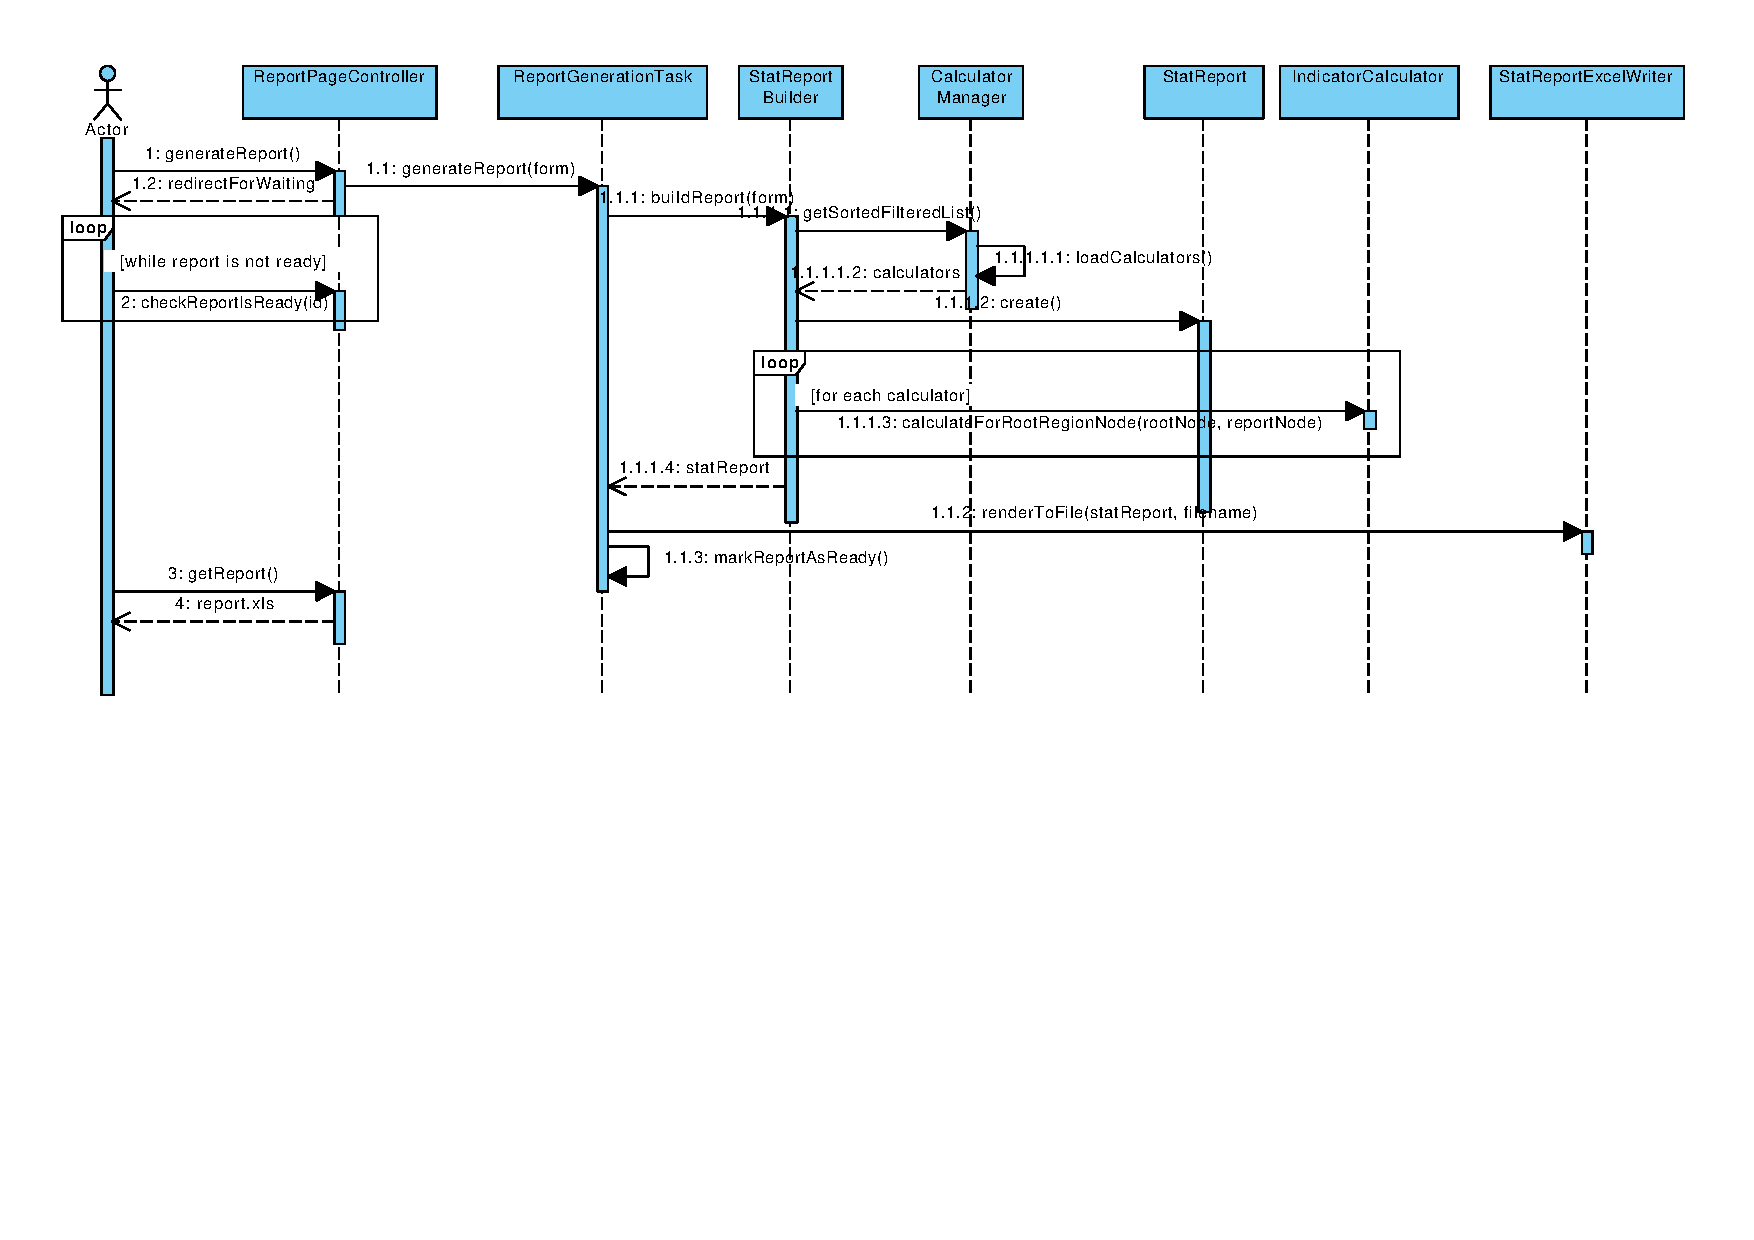
\includegraphics[scale=0.60, trim=00mm 90mm 00mm 10mm, clip]{../resources/uml/ReportCreation.pdf}
\caption{Диаграмма последовательности для процесса создания отчета}
\label{gr:report_creation}
\end{center} 
\end{figure}

В общем случае генерация отчета инициируется пользователем на странице с формой отчета, 
запрос поступает на обработку в \textit{ReportPageController}, где запускается фоновая задача
\textit{ReportGenerationTask}, а браузер пользователя перенаправляется на страницу ожидания,
где с помощью регулярных Ajax-запросов устанавливается, закончился ли процесс создания.
После того, как отчет сгенерировался браузер пользователя начинает его скачивать.

Обязанность объекта класса \textit{ReportGenerationTask} заключается в том, чтобы 
вызвать метод \textit{buildReport()}, класса \textit{StatReportBuilder}, передав 
параметры формы. Результатом работы этого метода должен стать отчет --- объект класса \textit{StatReport},
который потом необходимо сохранить в виде файла формата Excel, и закончить выполнение задачи.

\textit{StatReportBuilder} получает у класса \textit{CalculatorManager} список объектов
класса \textit{IndicatorCalculator} --- объекты-вычислители показателей, после чего
для каждого из них вызывает метод для добавления соответствующего показателя в отчет.

\subsubsection{Вычислители показателей}
\begin{figure}[!ht]
\begin{center}
\vspace{-0.4cm}
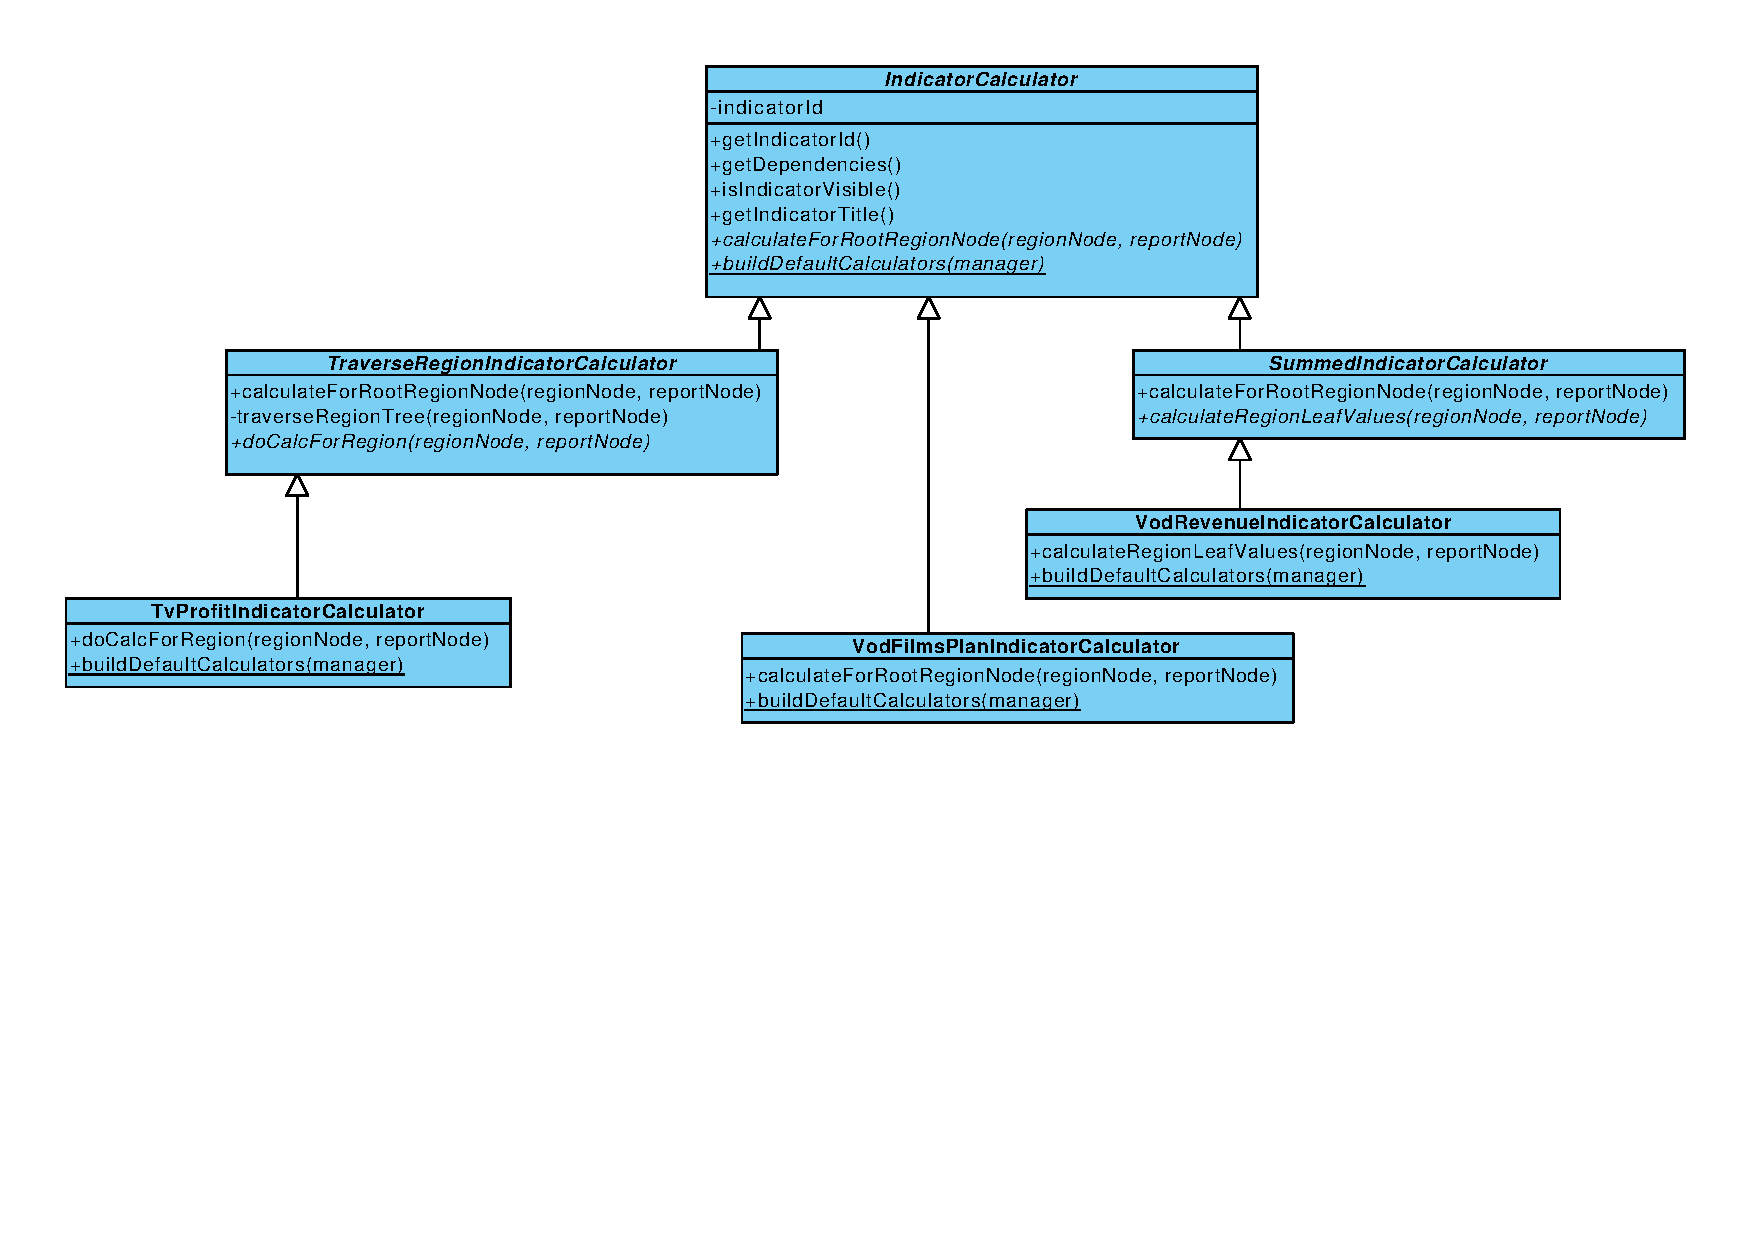
\includegraphics[scale=0.60, trim=00mm 80mm 00mm 10mm, clip]{../resources/uml/StatReportIndicatorCalculator.pdf}
\caption{Классы вычислителей}
\label{gr:report_creation}
\end{center} 
\end{figure}

Каждый из показателей, описанных в \ref{reports:indicators}, должен быть расчитан одним из объектов
иерархии классов \textit{IndicatorCalculator}. В ходе проектирования было выделено три основных типа
показателей:
\begin{enumerate}
\item{
  Показатели, которые не зависят от положении в дереве регионов и имеют смысл только в 
контексте корня дерева (например ``Количество ассетов''), классы для таких показателей
наследуются от \textit{IndicatorCalculator}, реализуя метод вычисления для корневой вершины. 
}
\item{
  Показатели, которые вычисляются для листьев дерева регионов, значения для всех остальных территорий
расчитываются как суммы значений потомков. Классы наследуются от \textit{SummedIndicatorCalculator}
и реализуют метод вычисления для листьев.
}
\item{
  Показатели, которые вычисляются для каждой вершины дерева регионов независимо.
В этом случае классы наследуются от \textit{TraverseRegionIndicatorCalculator} и 
и реализуют метод вычисления для каждой вершины.
}
\end{enumerate}

В реализациях метода \textit{calculateForRootRegionNode()} классов \textit{SummedIndicatorCalculator} и \textit{TraverseRegionIndicatorCalculator} 
описана соотвествующая логика для обхода дерева регионов и суммирования значений.

Следует учитывать, что некоторые из показателей расчитываются на основании значений других показателей,
например ``Прибыль'' расчитывается на основе ``Выручки'' и ``Отчислений'', в связи с этим запускать
вычислители необходимо в определенном порядке, чтобы зависимые показатели не начинались расчет перед
основными.

Любой объект вычислитель обладает присвоенным идентификатором показателя, уникальным в рамках работы построителя отчетов.

\begin{figure}[!ht]
\begin{center}
\vspace{-0.2cm}
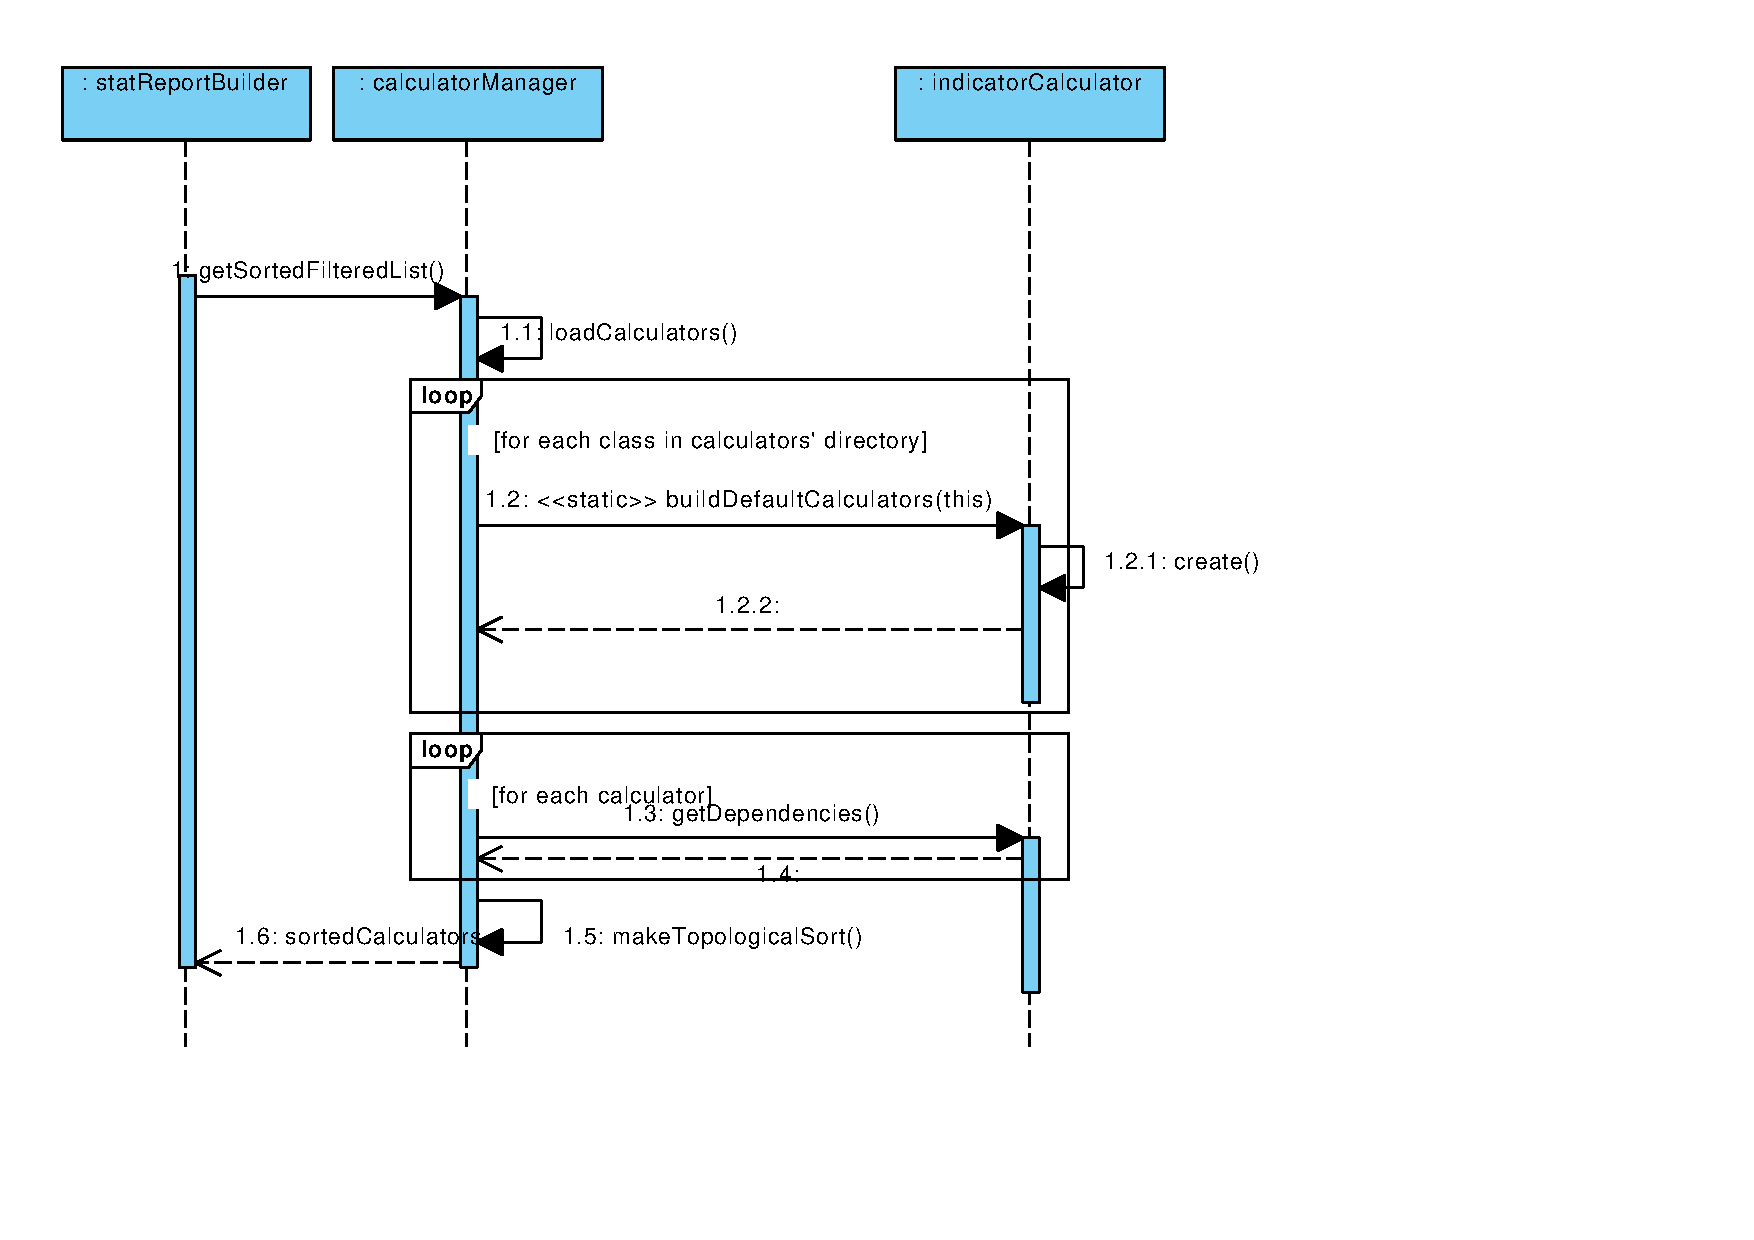
\includegraphics[scale=0.50, trim=00mm 30mm 00mm 10mm, clip]{../resources/uml/CalculatorLoading.pdf}
\caption{Загрузка вычислителей}
\label{gr:report_creation}
\end{center} 
\end{figure}

\paragraph{Загрузка вычислителей} Для упрощения создания новых вычислителей, а также для упрощения работы
с зависимыми показателями было создано следующее архитектурное решение:
\begin{enumerate}
\item{
  Когда построитель отчета (\textit{StatReportBuilder}) запрашивает у контроллера вычислителей
(\textit{CalculatorManager}) отсортированный список, последний объект загружает все файлы-классы
из определенных в конфигурационных файлах директорий.
}
\item{
  У каждого загруженного класса вызывается статичный метод \textit{buildDefaultCalculators()},
  который добавляет в объект-менеджер сконфигурированные экземляры соответствующего класса, в общем случае
их может быть больше одного.
}
\item{
  В интерфейсе класса вычислителей присутствует метод \textit{getDependencies()}, который возвращает
список уникальных идентификаторов показателей, от которых зависит данный объект. 
}
\item{
  На основе этих списков конструируется ориентированный граф зависимостей, после чего проверяется отсутствие
циклов и производится его топологическая сортировка.
}
\item{
  Таким образом в результате работы алгоритма менеджер возвращает построителю список объектов класса
\textit{IndicatorCalculator}, отсортированный таким образом, что если вызывать их в этом порядке,
не должна возникнуть ситуация, когда вычисление зависимых показателей вызывается до расчета основных.
}
\end{enumerate}

\paragraph{Добавление новых показателей} В случае появления требований, связанных с добавлением
нового вида показателей, разработчику необходимо:
\begin{enumerate}
\item{
  Определить вид нового показателя в соответствии с одним из трех типов, описанных в начале раздела. 
}
\item{
  Создать класс вычислителей, унаследовав его от одного из классов
\textit{IndicatorCalculator}, \textit{SummedIndicatorCalculator} или \textit{TraverseRegionIndicatorCalculator},
реализовав логику вычисления в соответствующих методах.
}
\item{
  Добавить в класс статический метод \textit{buildDefaultCalculators()}, в котором создаются и 
конфигурируются экземпляры данного класса вычислителей.
}
\item{
  В случае зависимости от других показателей необходимо перекрыть метод \textit{getDependencies()},
в котором следует возвратить список зависимостей.
}
\item{
  Следует поместить созданный класс в директорию с другими вычислителями, создав файл с именем \textit{<ClassName>.php},
  а также добавить в класс формы параметров отчета названия и идентификаторы новых показателей.
}
\end{enumerate}

\subsubsection{Оптимизация алгоритма расчета показателей}
Одной из важнейших характеристик модуля является время построения отчетов.
В этом разделе кратко описаны действия, предпринятые для оптимизации алгоритма расчета
показателей.

\paragraph{Сокращение числа запросов к СУБД}
В ходе экспериментальных исследований, связанных с замером времени выполнения различных операций
при построении отчета, было отмечено, что наиболее критичным параметром при работе с базой данных
является количество SQL-запросов. Время обработки 100 запросов, каждый из которых возвращает
одно значение, примерно в 20 раз превосходит время обработки результатов одного запроса,
возвращающего около одной тысячи значений.

Таким образом в рамках первой версии системы было принято решение сократить число запросов следующим образом:
\begin{itemize}
\item{
  Для каждой территории отчета нижнего уровня получать данные показателя
с помощью одного запроса для всех периодов и уровней детализации.
}
\item{
  В случае наличия данных только для листьев дерева регионов, и если выбрана 
неглубокая территориальная детализация (например по филиалам) вместо условия
равенства для региона использовать условие включения в множество потомков-листьев
для конкретной территории.
}
\item{
  Для получения данных по нескольким уровням детализации в рамках
одного запроса следует использовать конструкцию ``GROUPING SETS'',
представленную в рамках диалекта SQL для Microsoft SQL Server. 
Эта конструкция позволяет задавать группировку по нескольким полям
одновременно.
}
\end{itemize}

Для упрощения составления сложных запросов был реализован класс-компонент
\textit{StatReportQueryMaster}, метод которого 
\textit{calcAggregatedValuesForPeriods(model, indicators, periods, filters, keysSets, joins)}
конструирует запрос на основе переданного объекта-модели ``model'', списка 
значений-показателей ``indicators'' с учетом ограничений из ``periods'' и ``filters''.
Полученный запрос исполняется, а его результаты сохраняются в объект класса \textit{GroupResultSet},
инкапсулирующий доступ к группиророванным данным.

\paragraph{Использование индексов}
Очень важным фактором, влияющим на время выполнения запросов, является степень использования индексов.
При проектировании схемы должны быть учтены наиболее вероятно создаваемые типы запросов.

Например в случае запросов на выборку с фильтрацией и группировкой из таблицы с большим числом записей
необходим индекс, набор полей которого начинается с тех, которые задействованы в условии и продолжается
атрибутами, по которым происходит группировка. В этом случае, при использовании стандартных
агрегирующих функций \textit{COUNT(), MIN(), MAX()} возможно избежать полного просмотра таблицы.

При необходимости агрегации суммы будет выполнен частичный просмотр таблицы, а именно той части,
которая ограничена условиями. Для ускорения частичного просмотра оптимальным решением
является организация кластерного индекса таким образом, что его порядок совпадает с порядком
при фильтрации записей.

Индексы таблиц, используемых в ходе подготовки расчетов, спроектированы в соответствии
с этими требованиями.

\paragraph{Итоги}
В результате оптимизации время генерации полного отчета по Live со всеми выбранными показателями,
территориями и максимальным уровнем детализации составило порядка 15 минут с учетом числа записей
в таблицах со статистическими данными порядка 20 миллионов.

\subsubsection{Сохранение отчета в формате Excel}
%%todo: добавить скрин
При работе с файлами формата Microsoft Excel используется библиотека PHPExcel\cite{phpexcel},
распространяемая по лицензии GNU LGPL. Компоненты библиотеки предлагают интерфейсы, как
для чтения, так и для создания новых электронных таблиц с возможностью устанавливать
настройки форматирования документов для любых типов файлов, с которыми работает Microsoft Excel.

Для сохранения отчетов в xls-файл выделен отдельный компонент \textit{StatReportExcelWriter}
с единственным публичным методом \textit{renderToFile()}, принимающим в качестве аргументов уже
сформированный объект отчета и путь до файла, в который его нужно сохранить.
Выделение этого компонента позволяет отделить логику формирования отчета от его представления, 
в результате добавление другого формата вывода отчета пользователю, не должно вызвать особых 
сложностей даже в случае, если его природа сильно отличается от табличного представления.

В общем виде алгоритм сохранения реализован следующим образом:
\begin{enumerate}
\item{
  Вычисляется высота дерева показателей, эта информация используется для определения колонок, в которые будут выведены
значения показателей.
}
\item{
  Заполняется первая строка таблицы: записываются даты, определяющие периоды отчета, настраивается форматирование
для столбов показателей.
}
\item{
  Генерируется список вершин дерева в порядке обхода в глубину.
}
\item{
  Каждая вершина полученного списка выводится на отдельной строке, для каждого из типов вершин
предусматривается отдельный метод, определяющий формат и содержимое конкретной строки.
}
\item{
  В случае наличия нескольких валют, для которых был расчитан конкретный показатель, значения в валютах выводятся в 
  отдельных строках.
}
\end{enumerate}


